\appendix{Представление графического материала}

Графический материал, выполненный на отдельных листах,
изображен на рисунках А.1--А.\arabic{числоПлакатов}.
\setcounter{числоПлакатов}{0}

\renewcommand{\thefigure}{А.\arabic{figure}} % шаблон номера для плакатов

\begin{landscape}

\begin{плакат}
    
\includegraphics[width=0.82\linewidth]{svedenia.eps}
    \заголовок{Сведения о ВКРБ}
    \label{svedenia:image}      
\end{плакат}

\begin{плакат}
    
\includegraphics[width=0.82\linewidth]{cel_razrab.eps}
    \заголовок{Цель и задачи разработки}
    \label{cel_razrab:image}      
\end{плакат}

\begin{плакат}
    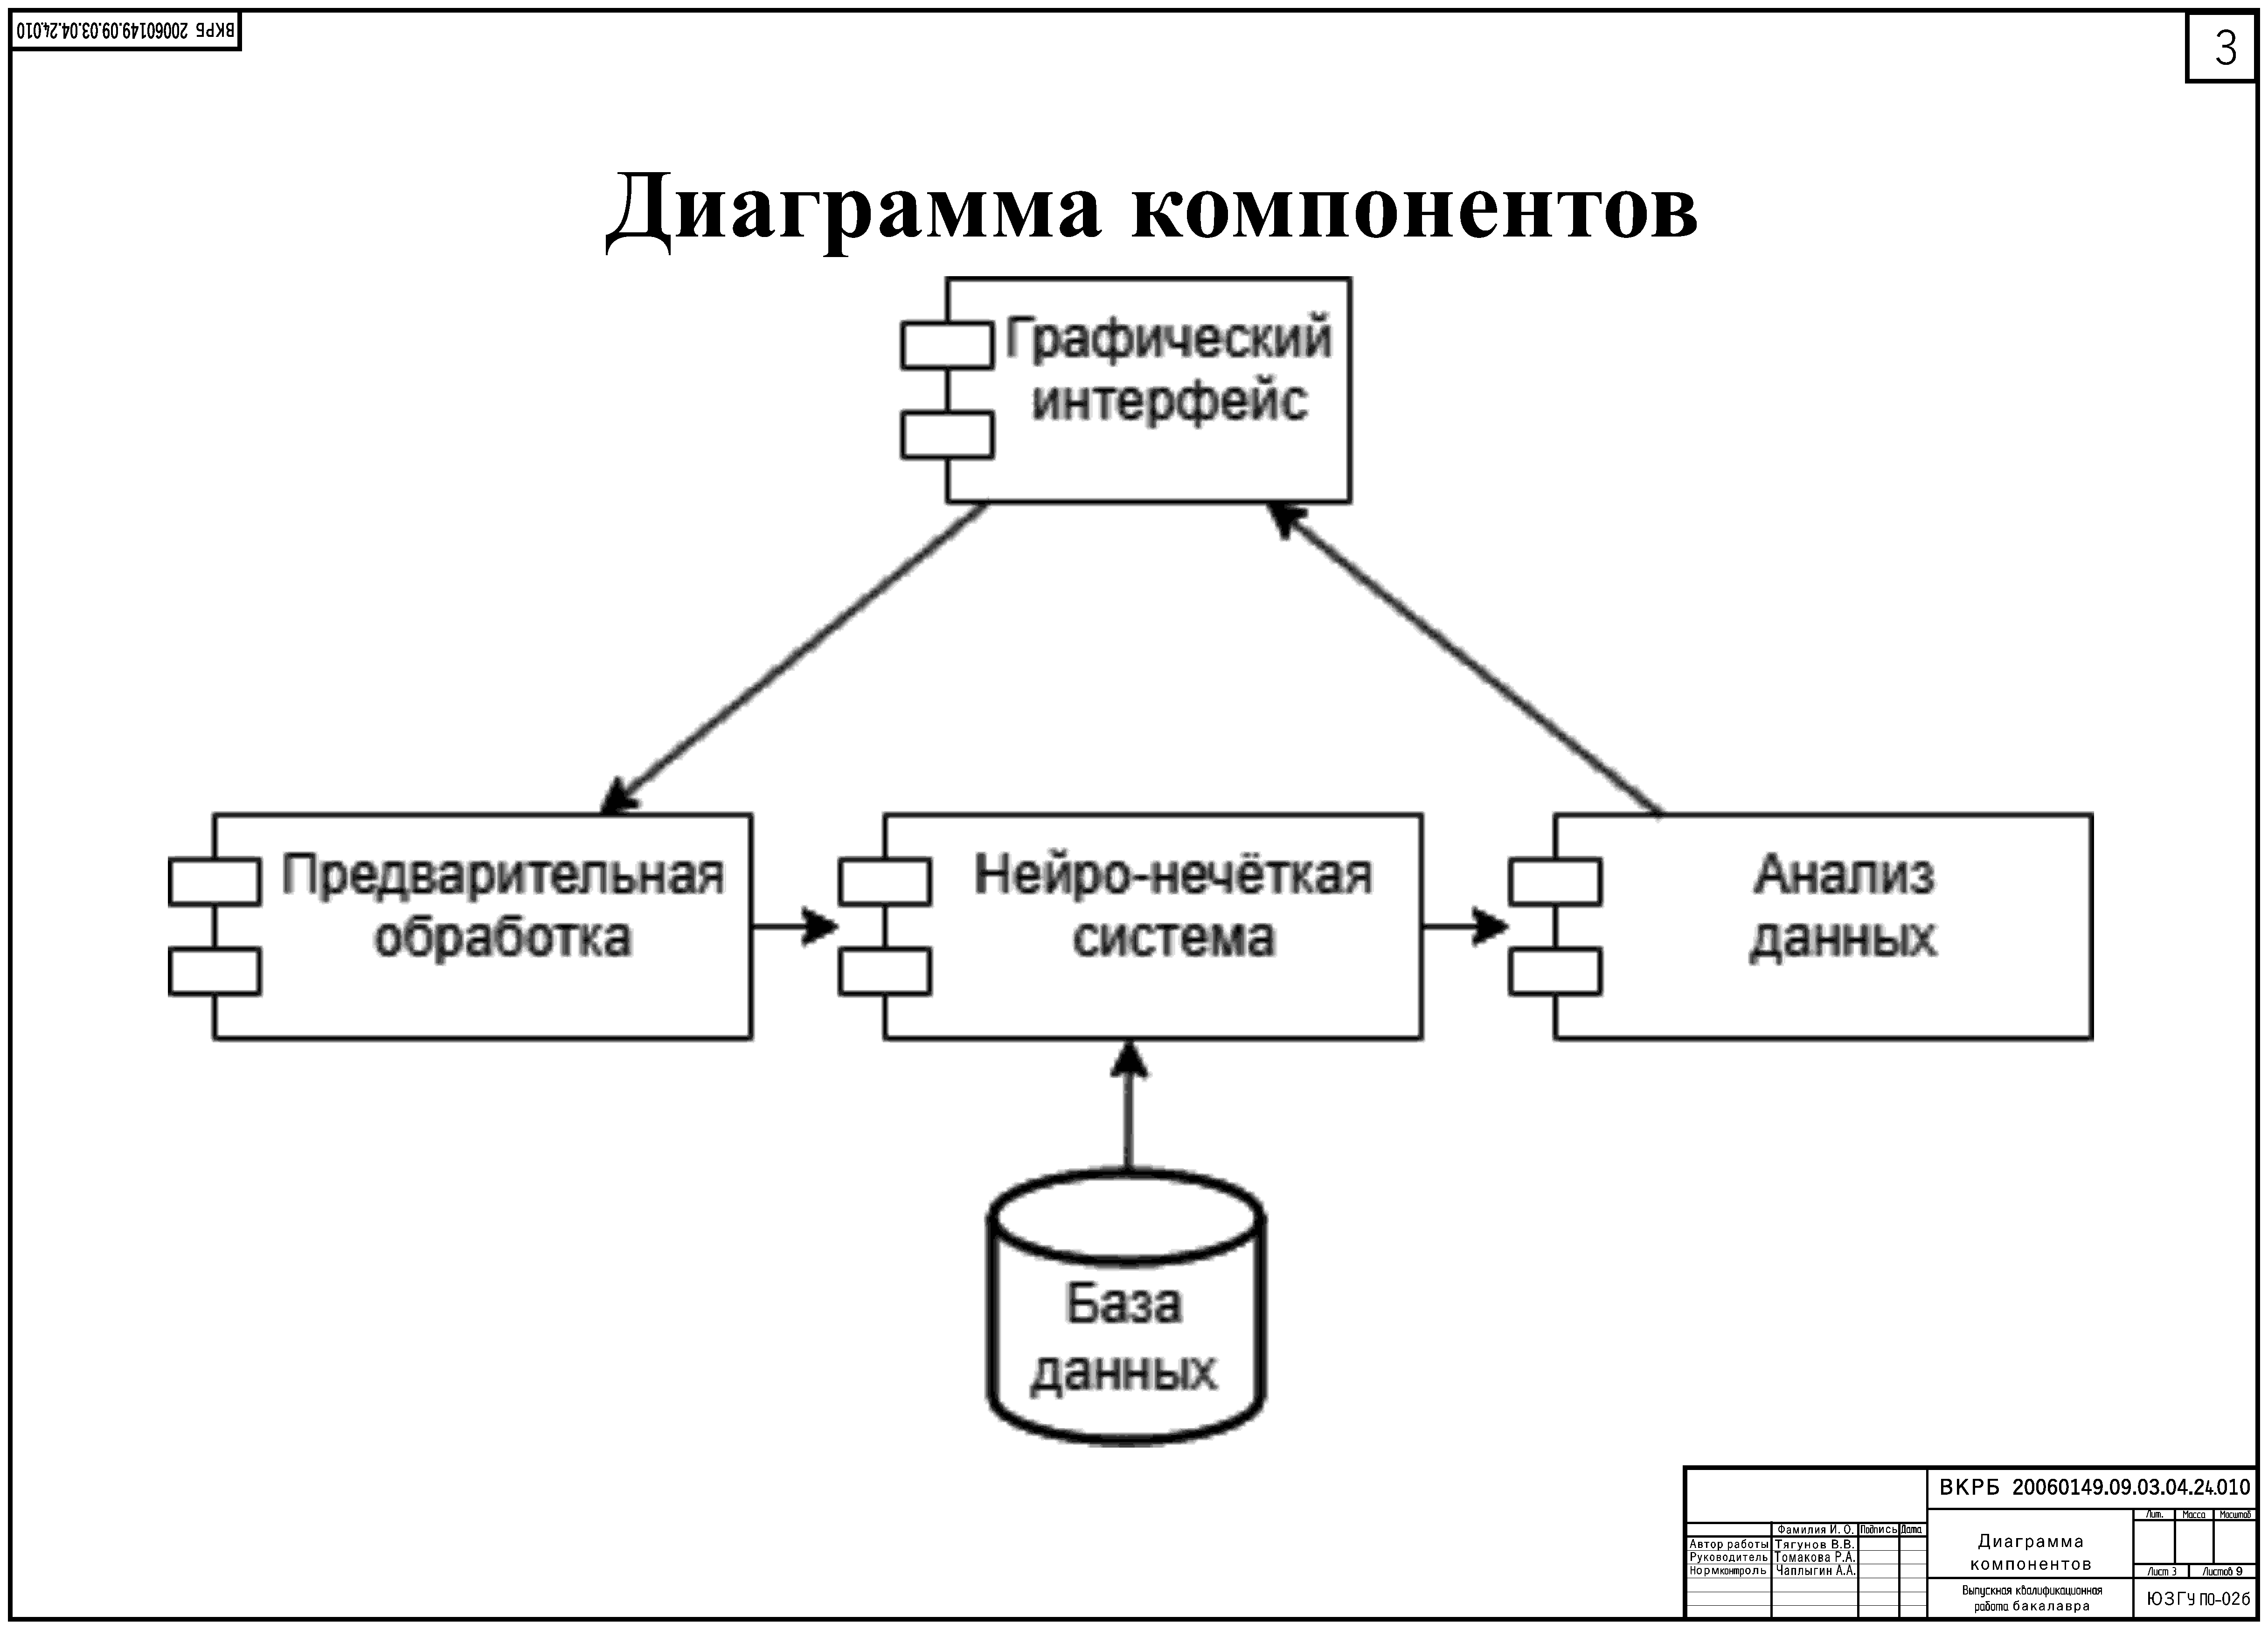
\includegraphics[width=0.82\linewidth]{comp_diagram_plakat.eps}
    \заголовок{Диаграммы компонентов}
    \label{comp_diagram_plakat:image}      
\end{плакат}

\begin{плакат}
    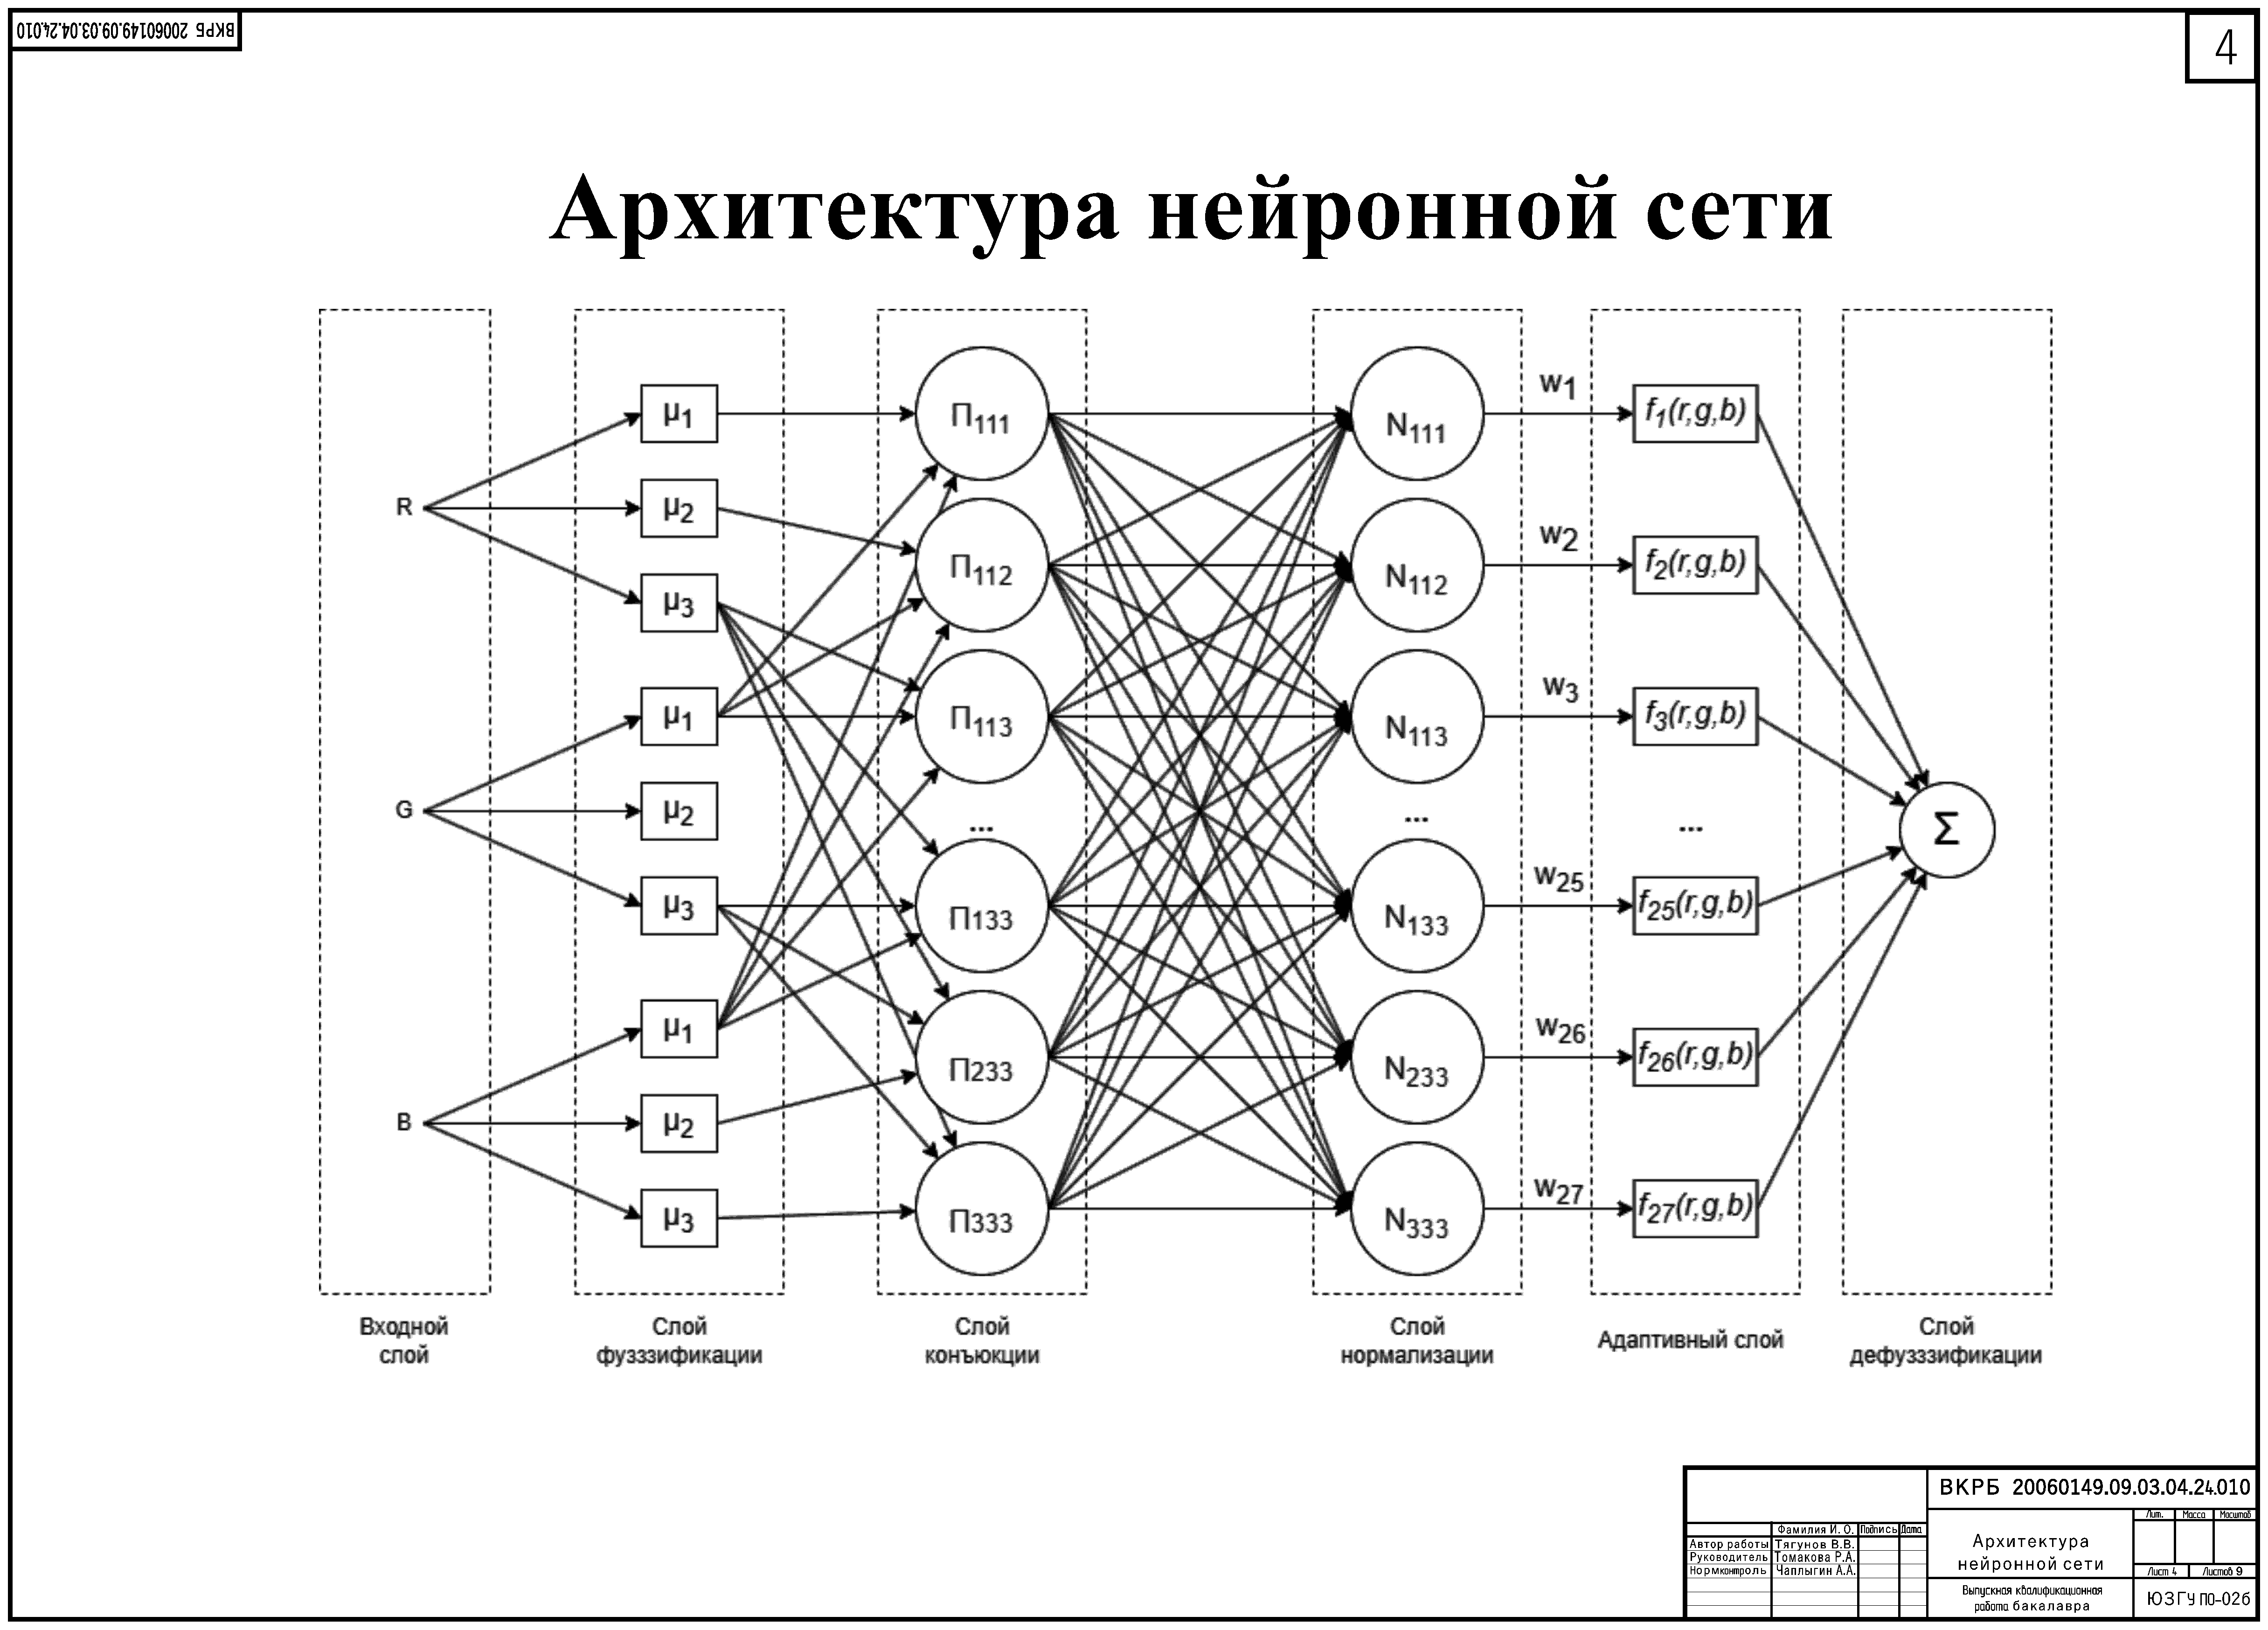
\includegraphics[width=0.82\linewidth]{ns_plakat.eps}
    \заголовок{Архитектура нейронной сети}
    \label{ns_plakat:image}      
\end{плакат}

\begin{плакат}
    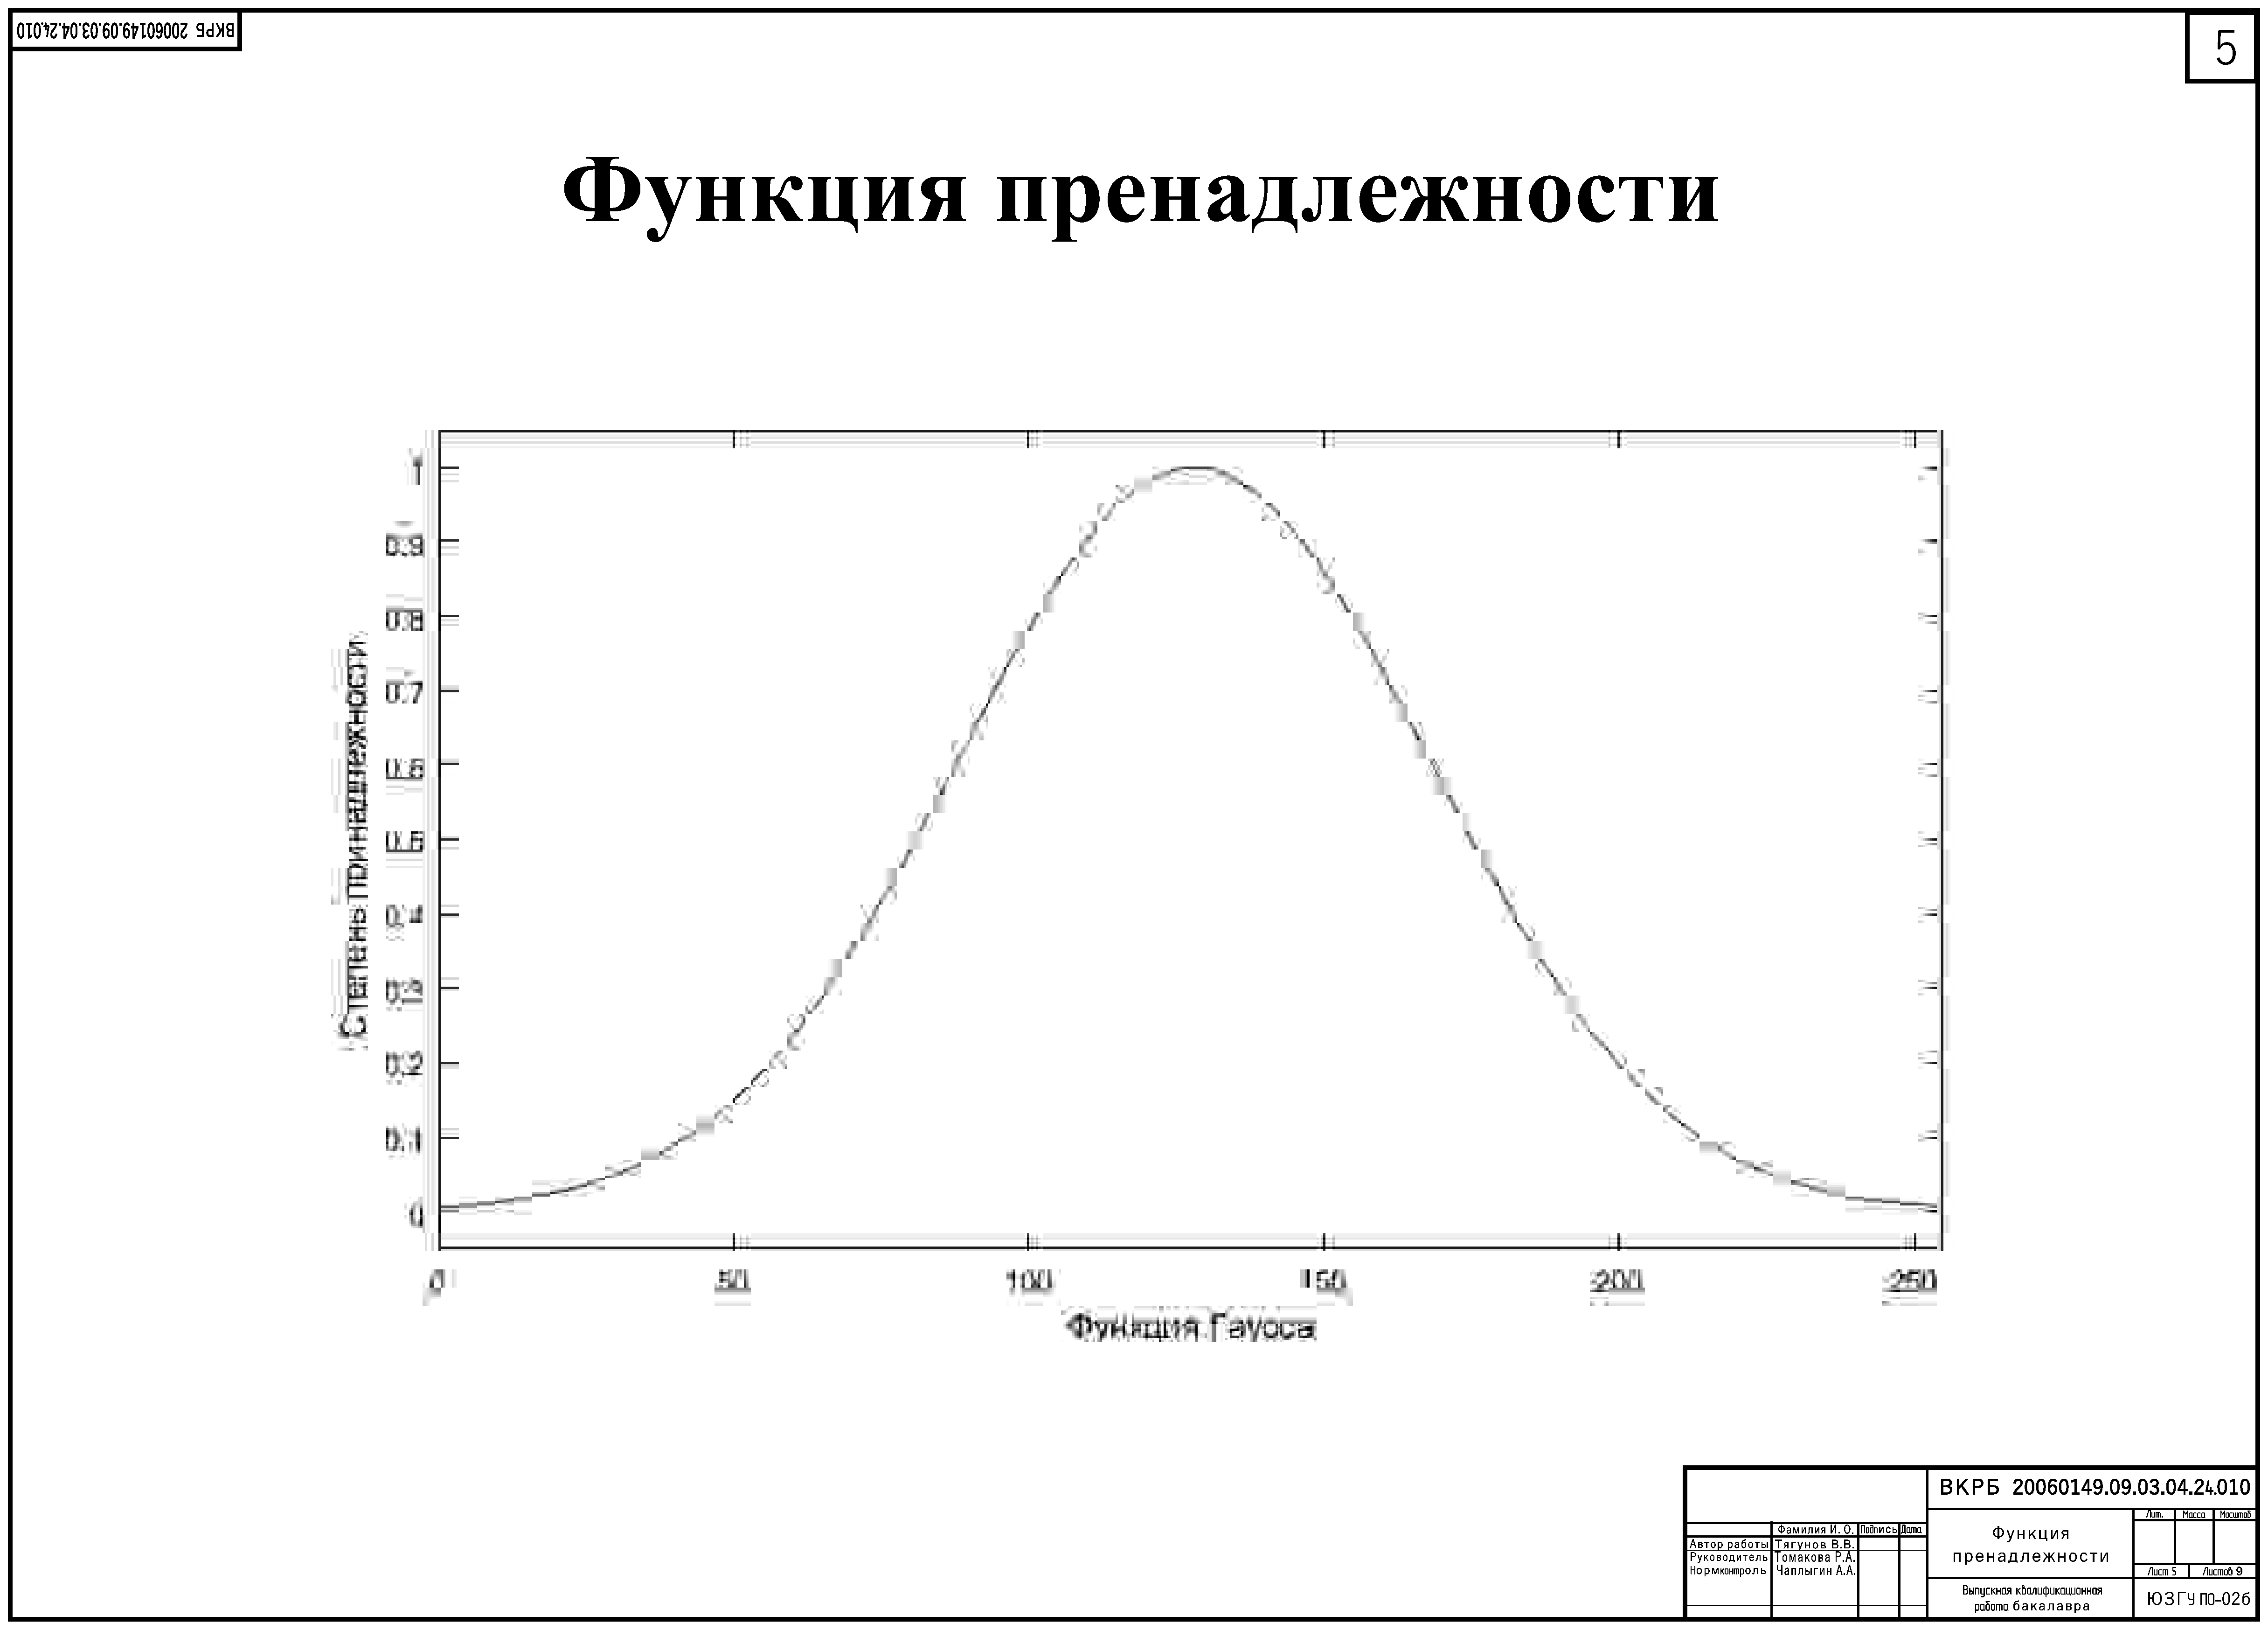
\includegraphics[width=0.82\linewidth]{funk.eps}
    \заголовок{Функция пренадлежности}
    \label{funk:image}      
\end{плакат}

\begin{плакат}
    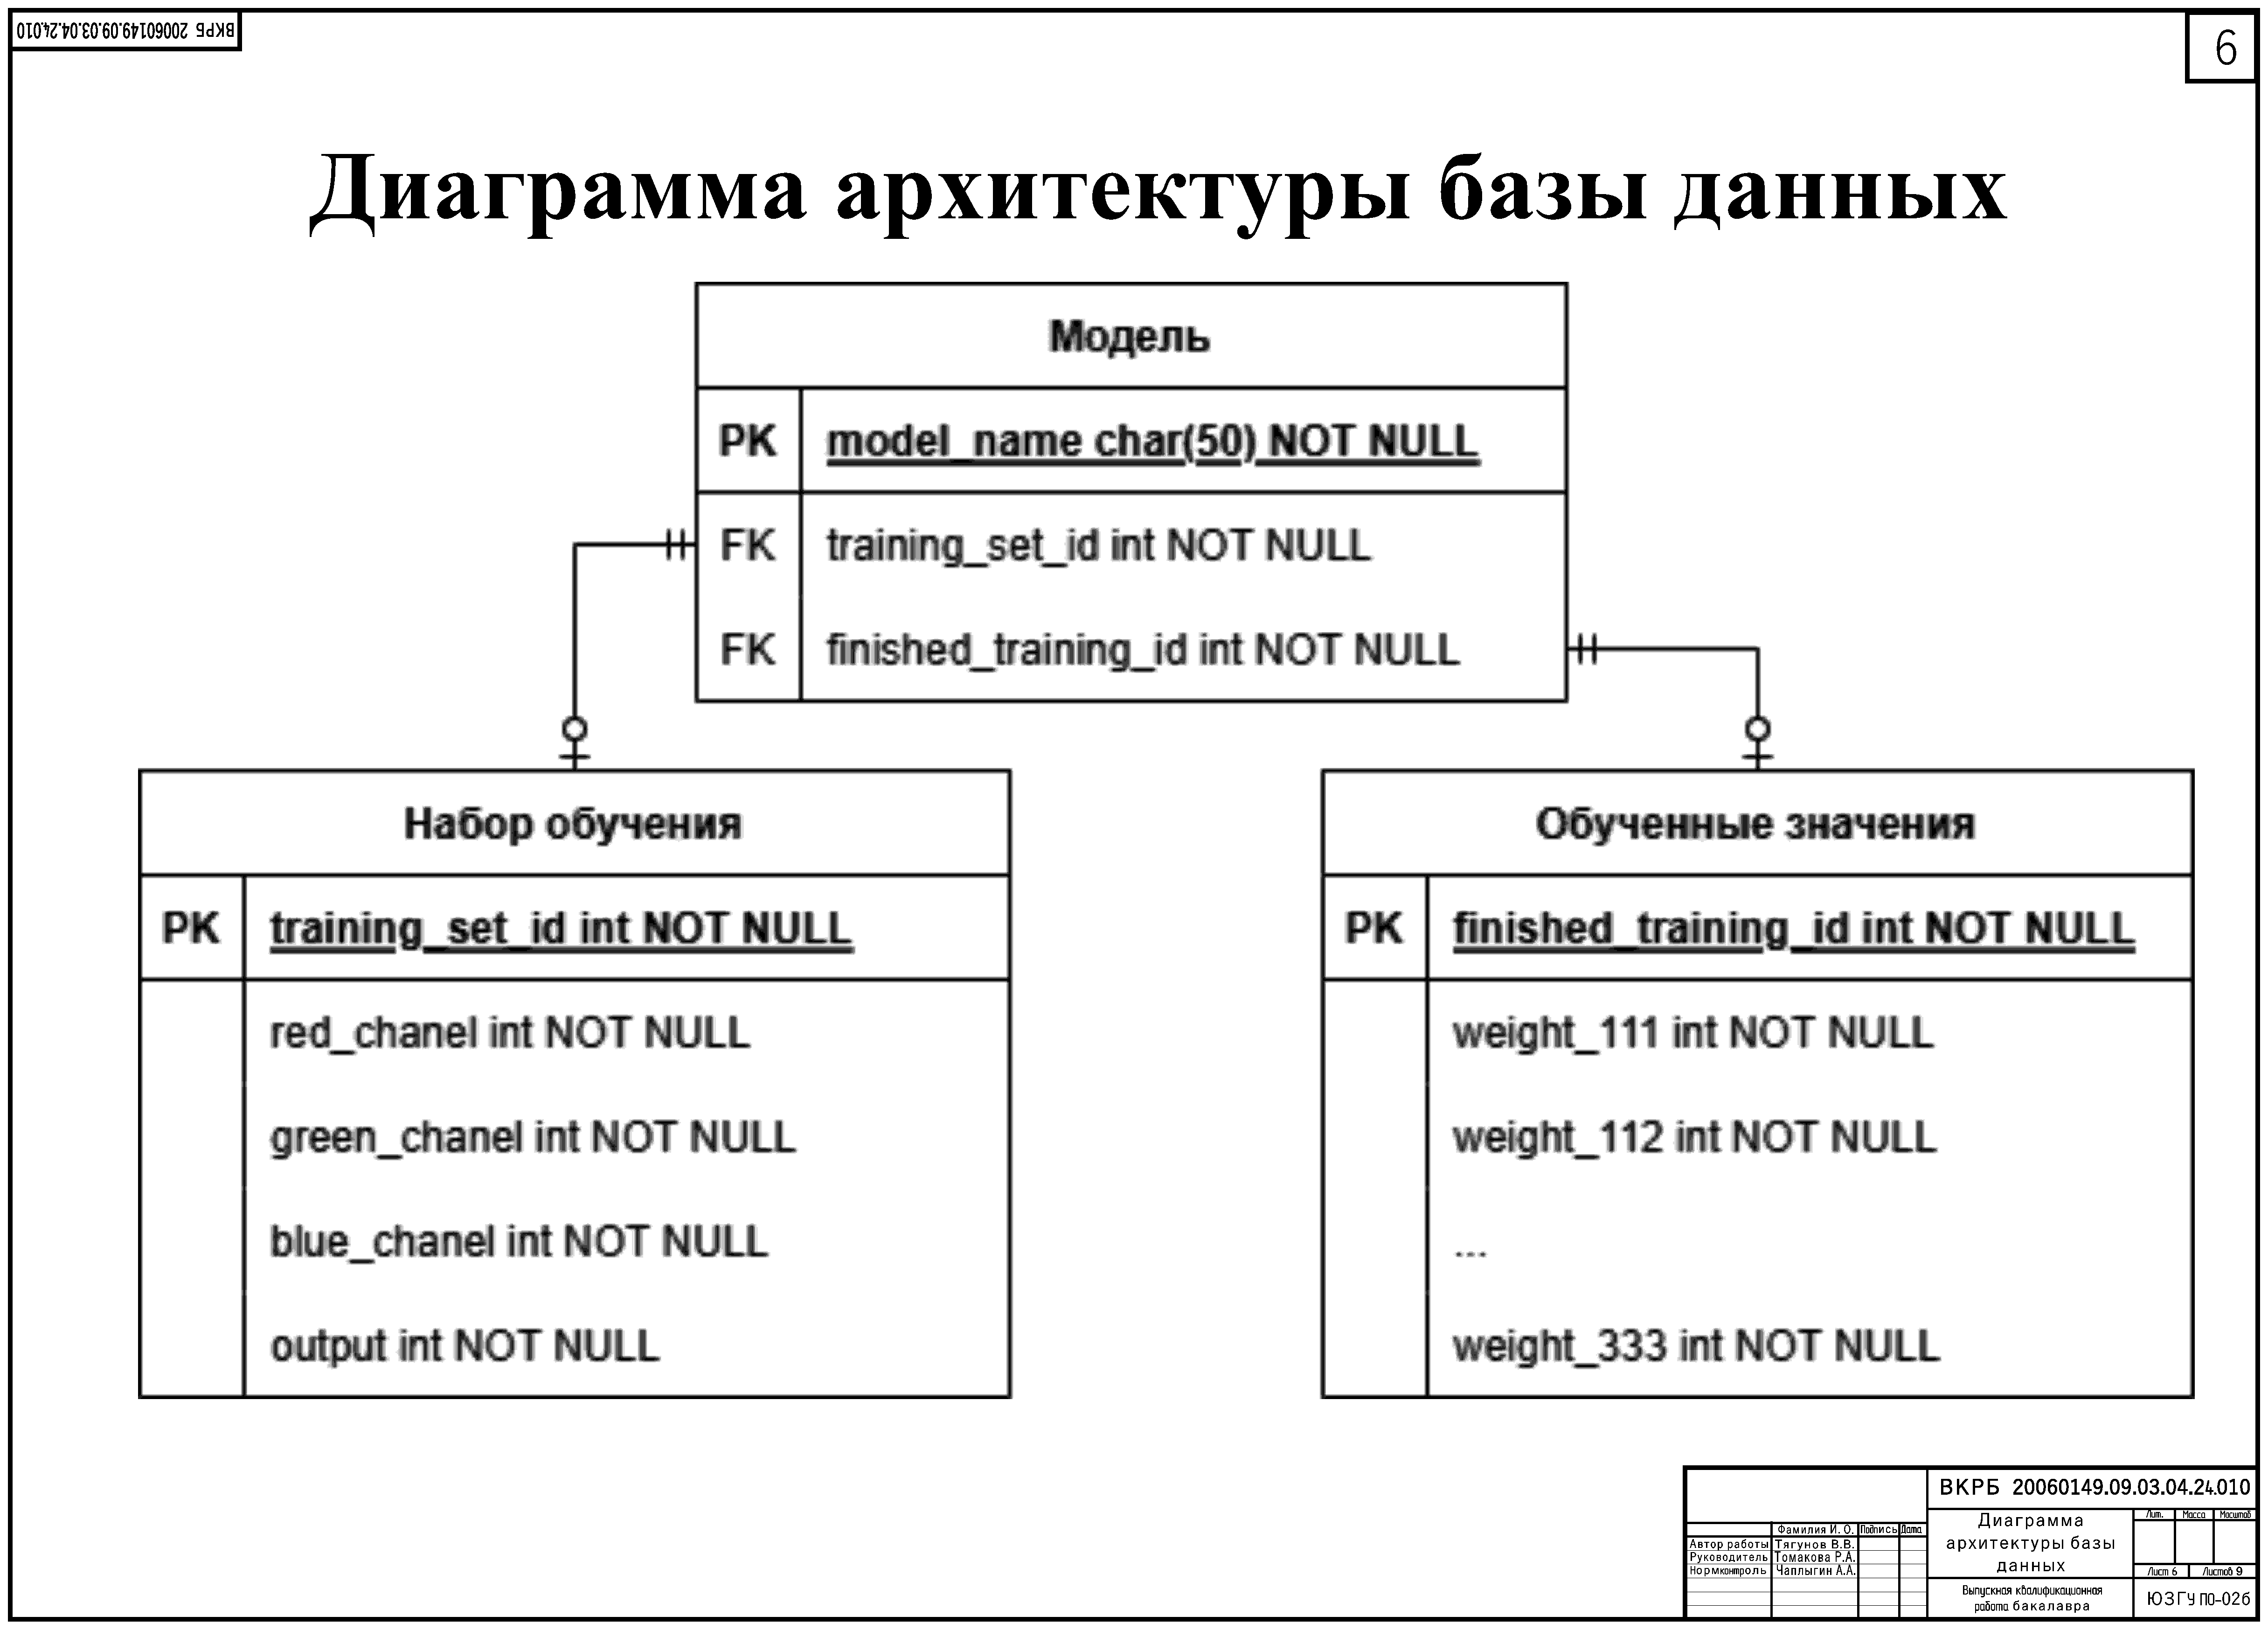
\includegraphics[width=0.82\linewidth]{BD_diagram_plakat.eps}
    \заголовок{База данных}
    \label{BD_diagram_plakat:image}      
\end{плакат}

\begin{плакат}
    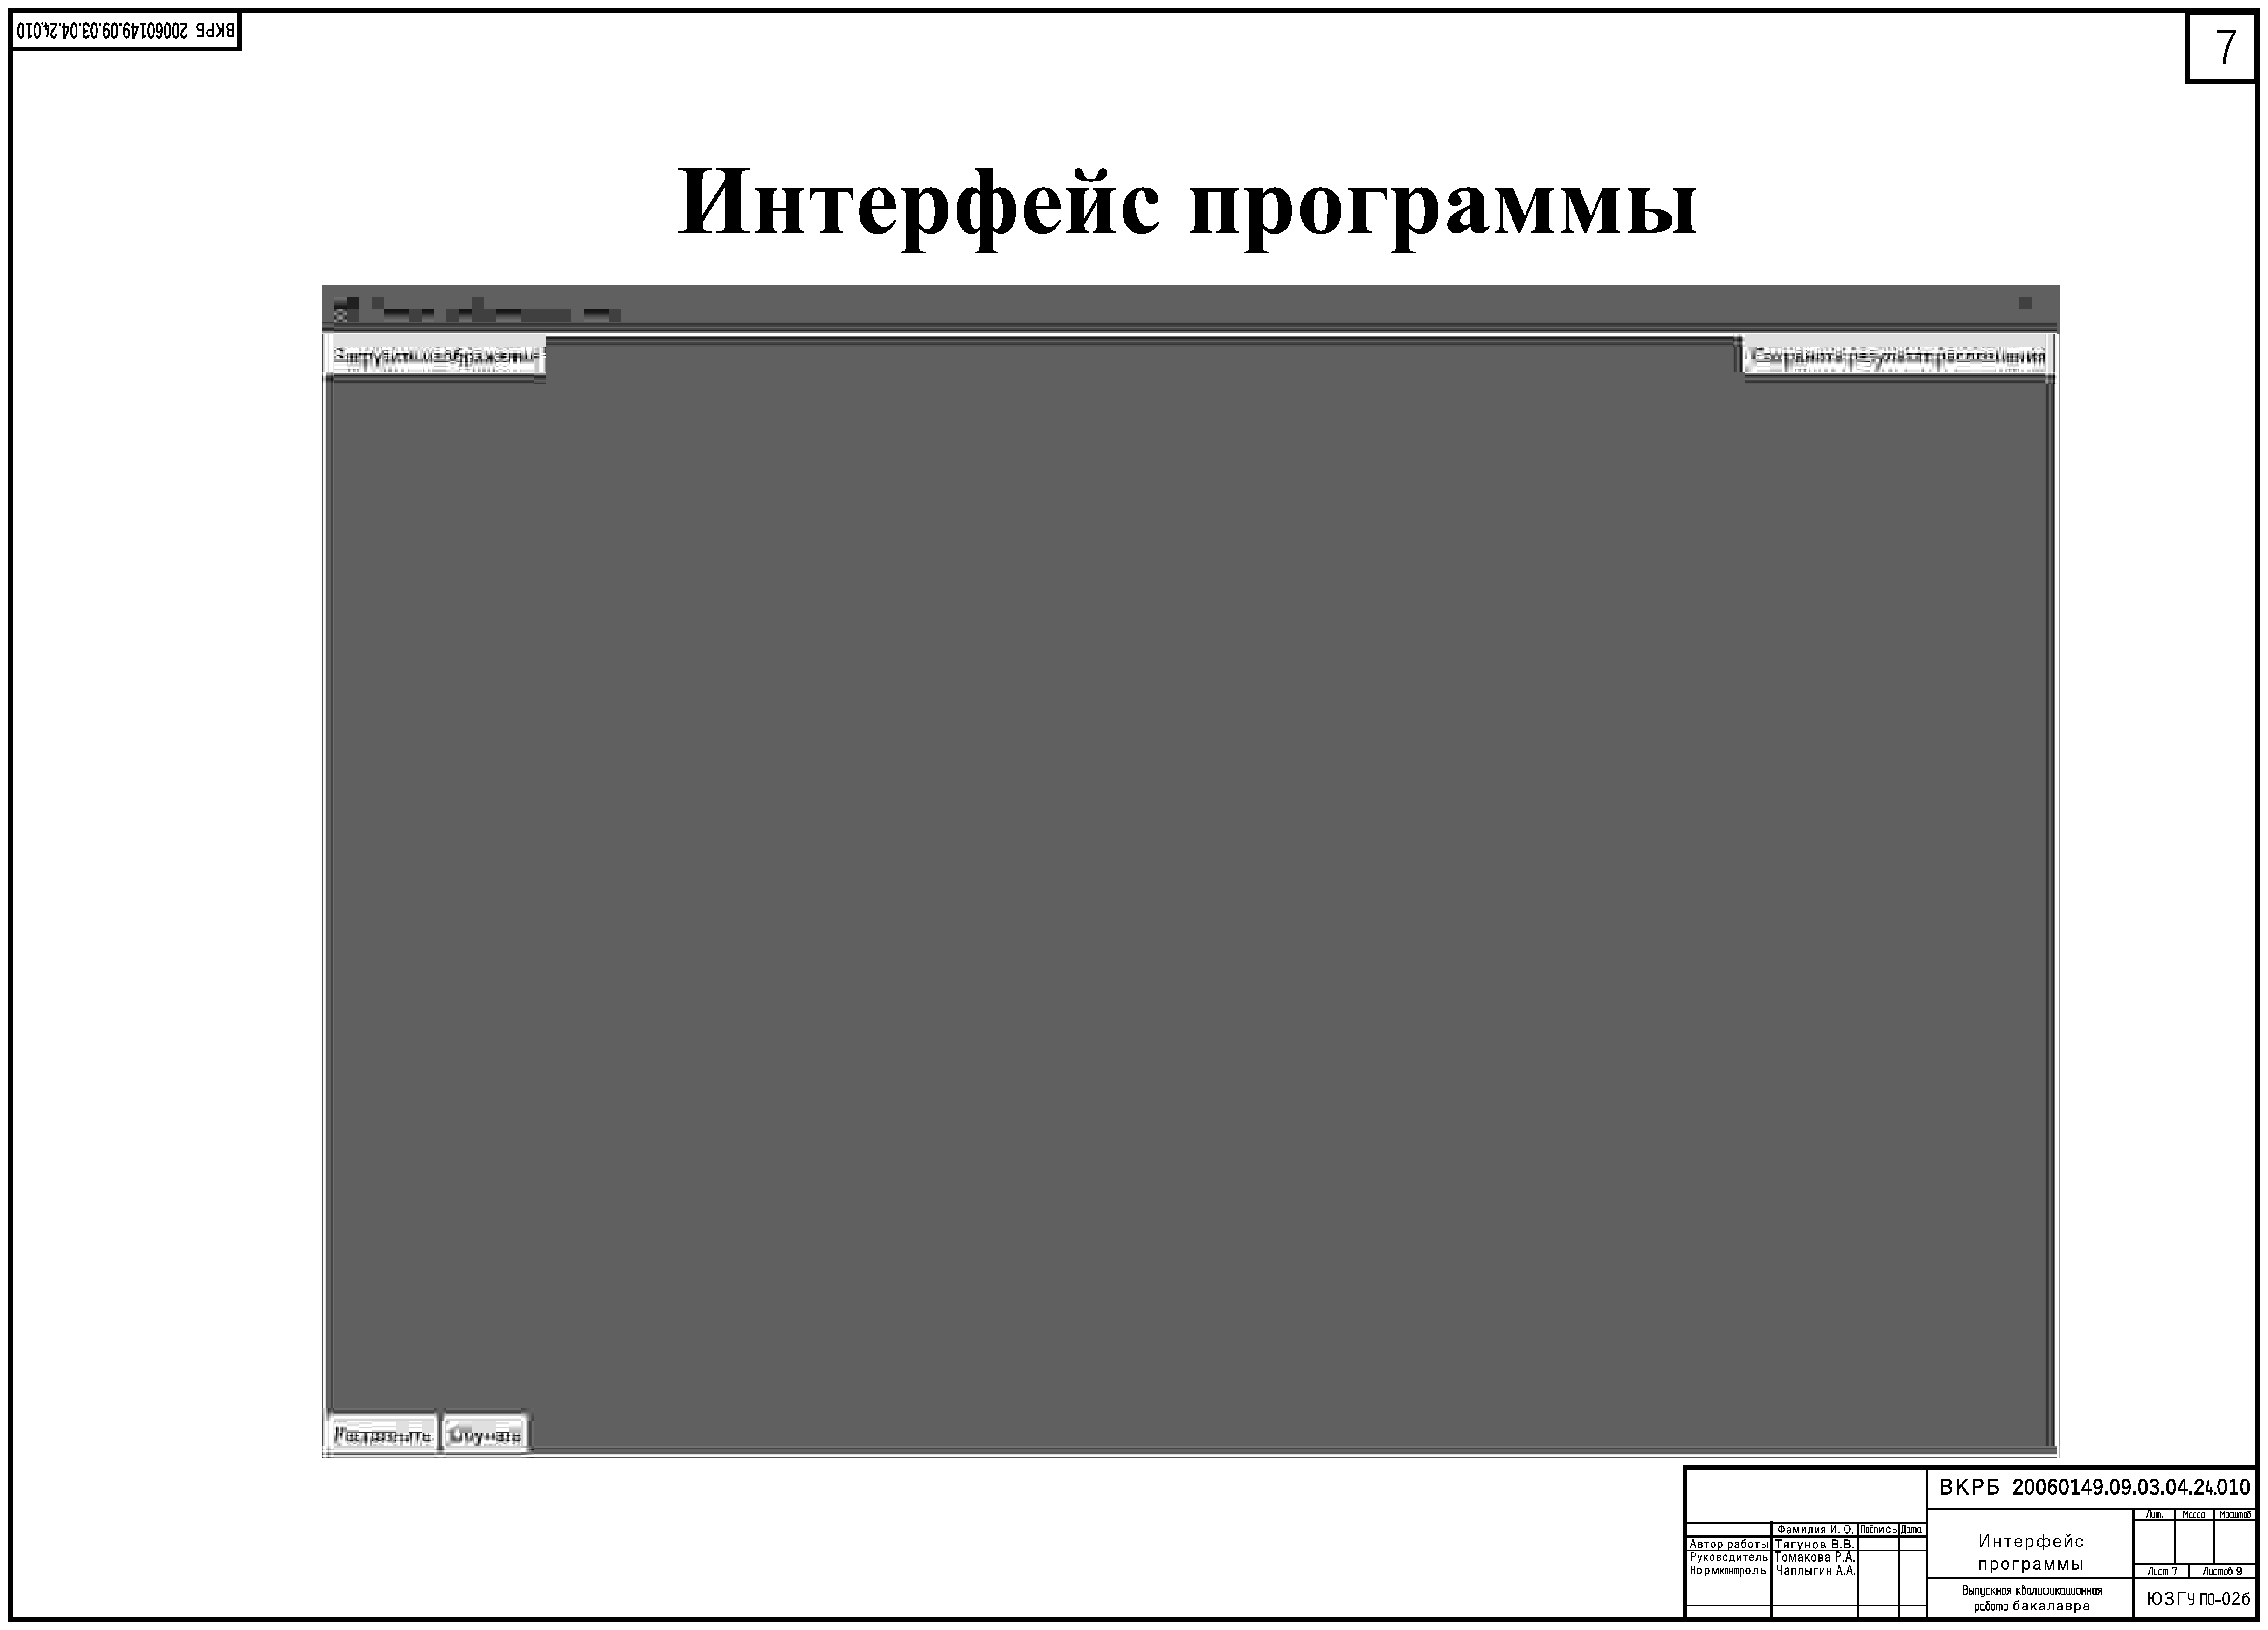
\includegraphics[width=0.82\linewidth]{program_interface_plakat.eps}
    \заголовок{Интерфейс приложения}
    \label{program_interface_plakat:image}      
\end{плакат}

\begin{плакат}
    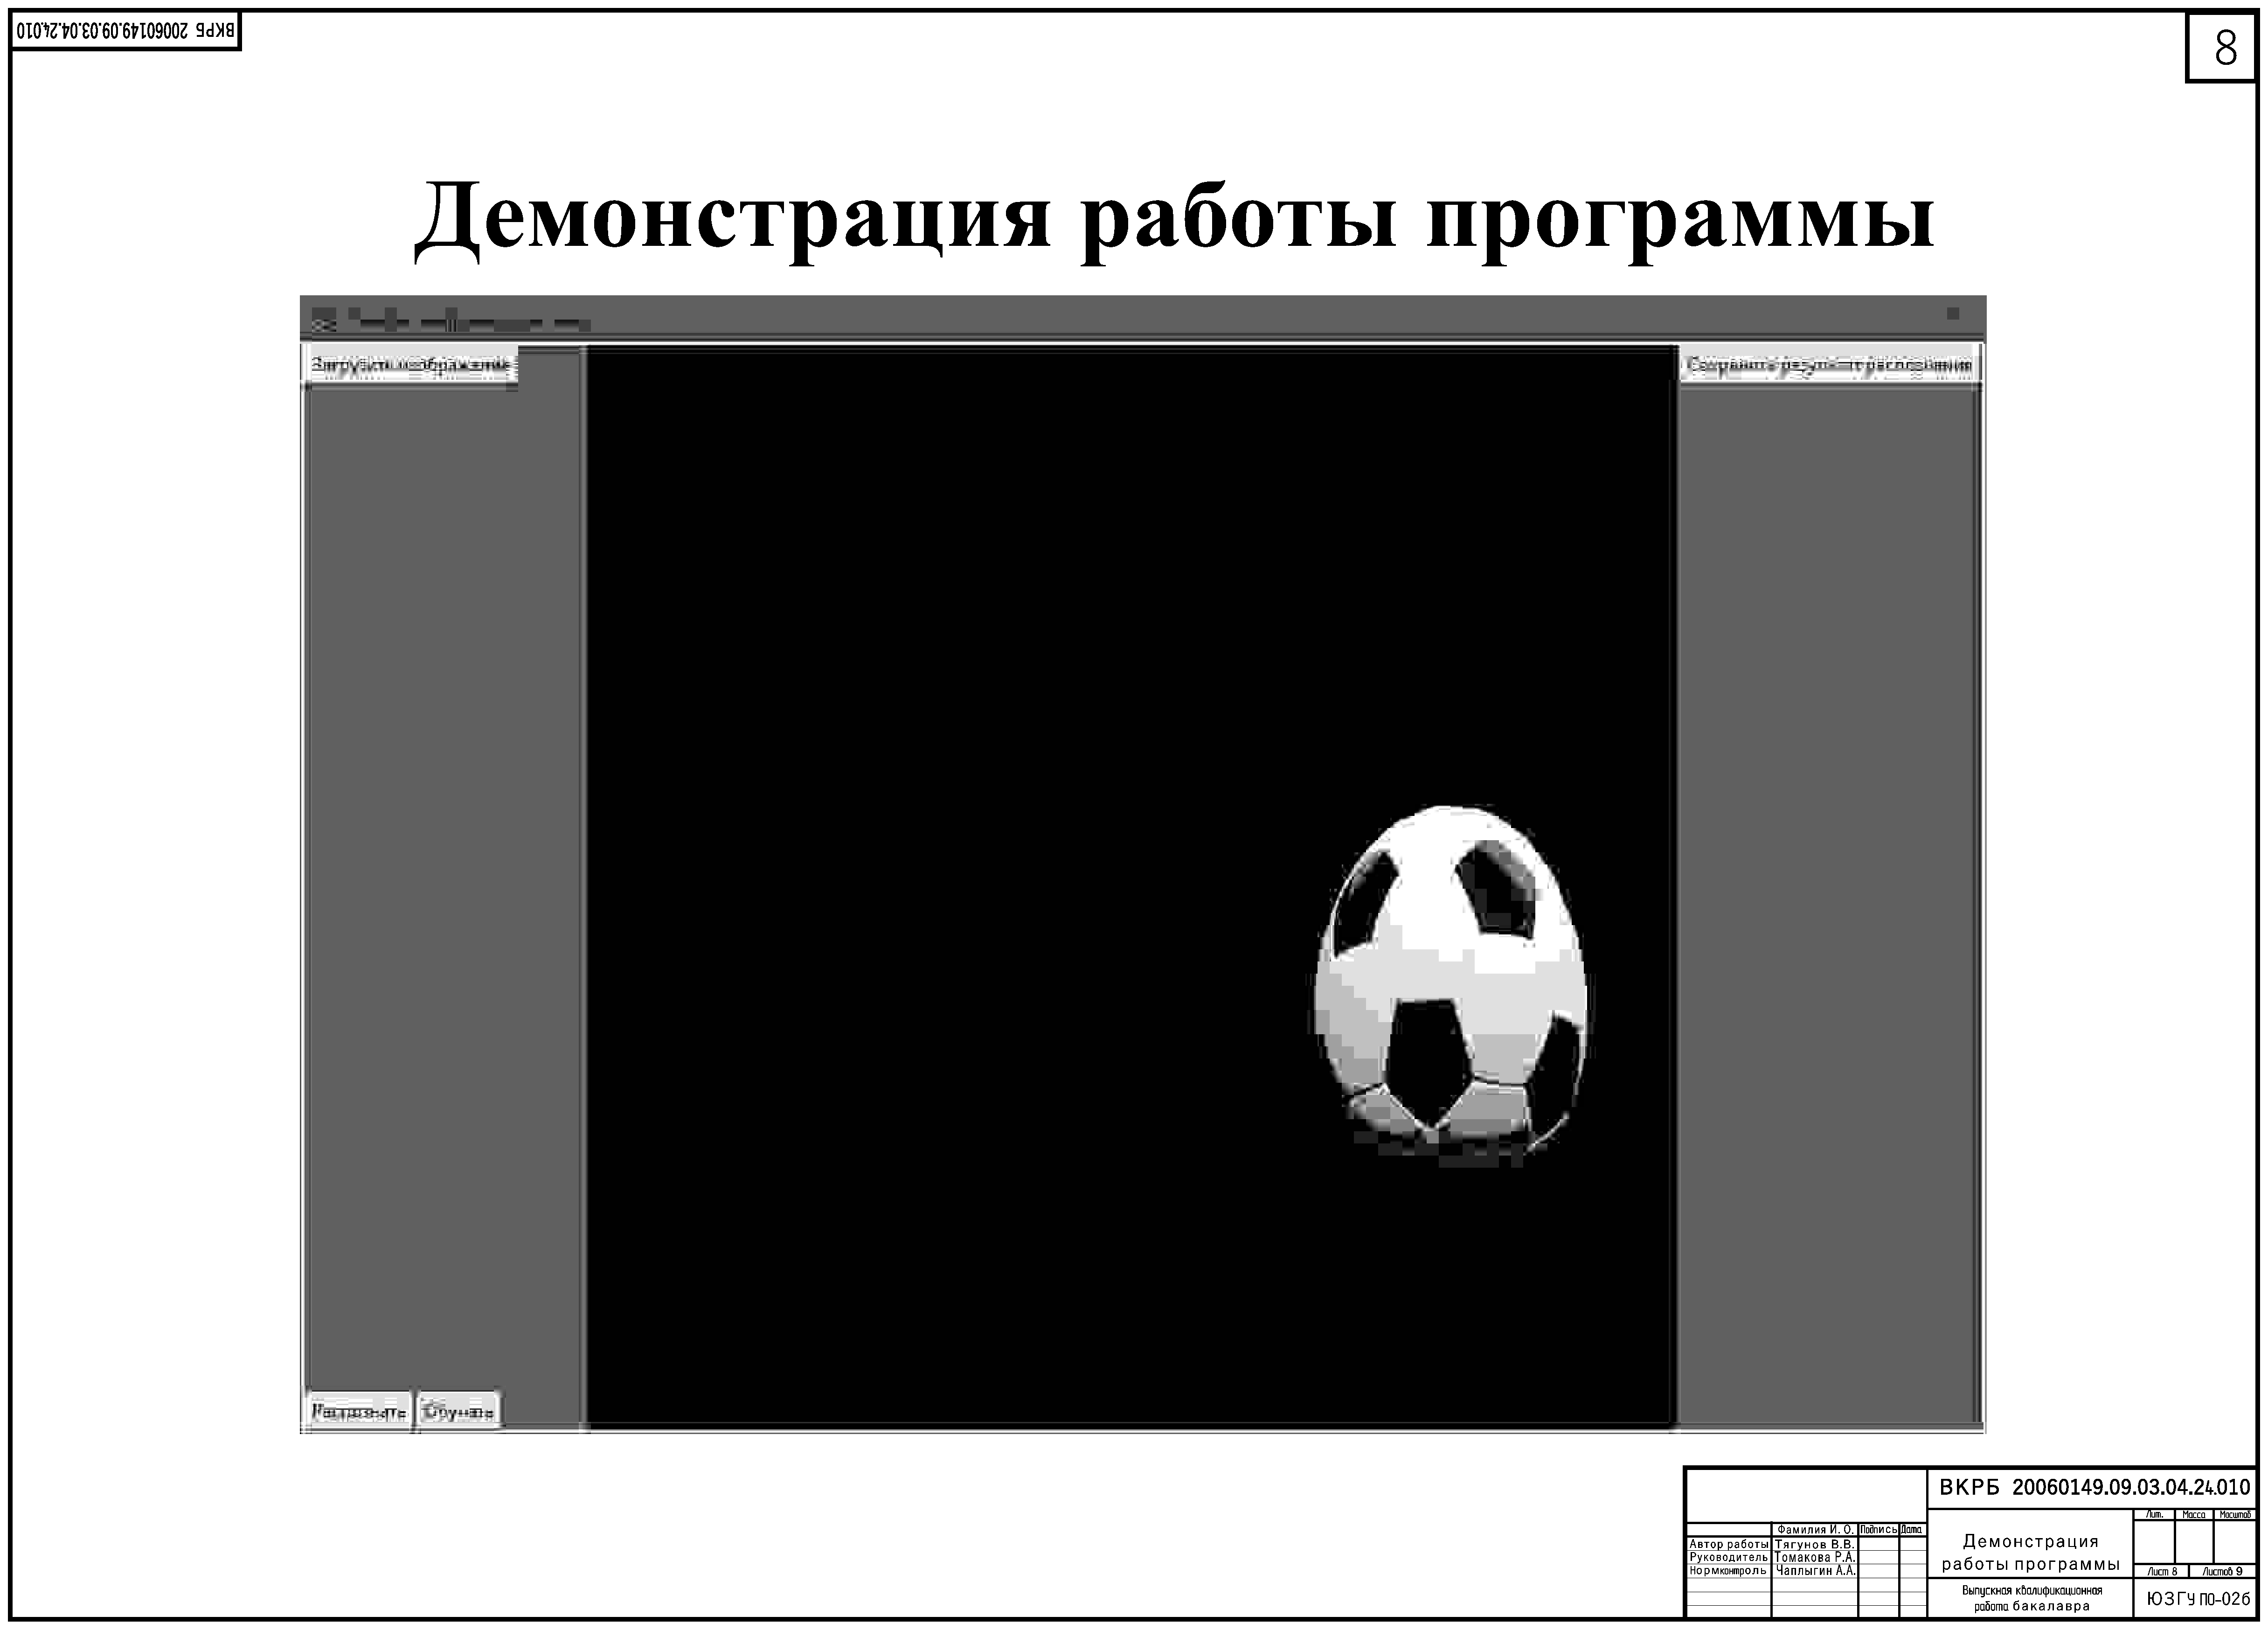
\includegraphics[width=0.82\linewidth]{rab.eps}
    \заголовок{Демонстрация работы программы}
    \label{rab:image}      
\end{плакат}

\begin{плакат}
    
\includegraphics[width=0.82\linewidth]{finish.eps}
    \заголовок{Заключение}
    \label{finish:image}      
\end{плакат}

\end{landscape}
